\newif\ifglobal

%%%%%%%%%%%%%%%%%%%%%%%
%%% Compile to view %%%
%%%%%%%%%%%%%%%%%%%%%%%

%%%%%%%%%%%%%%%%%%%%%%%%%%%%%%%%%%%%%%%%%%%%%%%%%%%
%%% Readme:                                     %%%
%%% https://www.overleaf.com/read/bwdjvfjksvjy/ %%%
%%%%%%%%%%%%%%%%%%%%%%%%%%%%%%%%%%%%%%%%%%%%%%%%%%%

% >>> M?: marks a module setting number or important notice

% >>> M4: Set {./relative-path} to external files for this module <<<
\def \modulefiles {./26-SDIOSLAVE}
% To add an external file, use:
% (Replace '---' with actual filename)
% '\input{\modulefiles/tables/---.tex}' for tables
% '\includegraphics{\modulefiles/figures/---}' for figures
% '\subfile{\modulefiles/---}' for register files


% >>> M1: This module is in global project? <<<
% 'YES' - uncomment; 'NO' - comment out
\globaltrue

\ifglobal
    \documentclass[main\_\_CN.tex]{subfiles}

\else
    % Font "FandolSong-Regular" used by ctex does not have GSUB table.
    % It causes warnings that do not affect compilation and can be ignored.
    \PassOptionsToPackage{quiet}{fontspec}

    \documentclass[openany, 10pt]{book}

    % >>> M2: In ./00-shared/preamble-trm-module, also find
    %         settings for visibility of todo notes, watermark <<<
    \usepackage{preamble-trm-module}

    % Enable Chinese typesetting
    \usepackage{ctex}

    % >>> M3: Temporary labels in Chinese
    %         you can add your own labels there <<<
    \myexternaldocument{./00-shared/temp-labels-cn}

\fi %\ifglobal


\setcounter{secnumdepth}{4}


% >>> M5: If this module needs any updates in
% './00-shared/preamble-trm-module.sty'
% (include additional package, etc.), contact your module PM
% or create the file './00-shared/changelog.tex' make the
% necessary updates yourself and document them in this file <<<

% Make text left-aligned and allow latex to break pages naturally, comment out for full justification
\raggedright
\raggedbottom


\begin{document}


% Sets language into which pre-defined bits of text are translated
\selectlanguage{chinese}
\setchineseformatting


% Do not delete this block
\ifglobal
% Add the following front matter if
% this module is outside of global project
\else
    \InputIfFileExists{readme}{}{}
    \listoftodos
    {\let\clearpage\relax \listofdonetodos}
    \tableofcontents
    %\listoftables
    %\listoffigures
\fi


%%%%%%%%%%%%%%%%%%%%%%%%%
%%% TRM Module Begins %%%
%%%%%%%%%%%%%%%%%%%%%%%%%

\hypertarget{sdioslave}{}
\chapter{SDIO 从机控制器 (SDIO)}
\label{mod:sdioslave}


\section{概述}
ESP32 支持数字输入输出 (SDIO) 设备接口，符合 SDIO 全速卡 V2.0 规范。主控器可以通过 SDIO 总线协议访问 ESP32。

主机 (Host) 可以直接访问 SDIO 接口寄存器，或通过使用 DMA 引擎访问设备上的共享存储器，在保证性能的同时减少了处理性能的浪费。

 \section{主要特性}
 \begin{itemize}
 \item 符合 SDIO 全速卡 V2.0 规范
    \item 支持 SDIO SPI，1-bit 和 4-bit 传输模式
    \item 0 \verb+~+ 50 MHz 时钟范围
    \item 可配置的采样时钟沿或驱动时钟沿
    \item 为信息交互设定的特定寄存器
    \item 支持自动填充 SDIO 总线上的发送数据，同样支持自动丢弃 SDIO 总线上的填充数据
    \item 高达 512 字节的块大小
    \item Host 与 Slave 间有中断向量可以相互中断对方
    \item 用于数据传输的 DMA
\end{itemize}
\section{功能描述}
\subsection{SDIO Slave 功能块图}
SDIO Slave 的功能块图如图 \ref{figure:SDIO Slave block diagram} 所示。

 \begin{figure}[H]
    \centering
    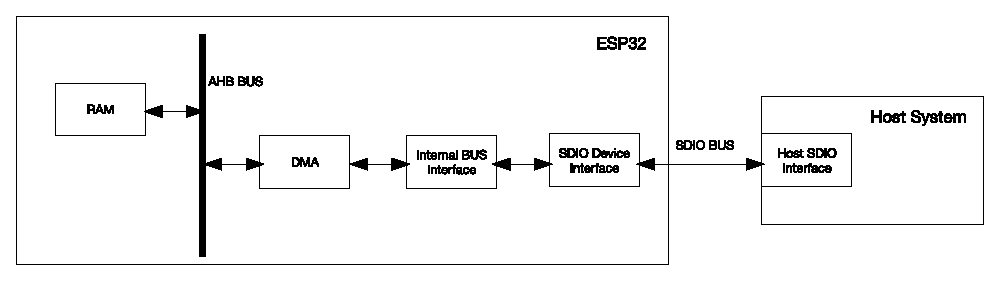
\includegraphics[width=0.9\textwidth]{./26-SDIOSLAVE/figures/SDIOSlaveBlockDiagram}
    \caption{SDIO Slave 功能块图}
    \label{figure:SDIO Slave block diagram}
\end{figure}

主机系统 (Host System) 代表任一符合 SDIO V2.0 规范的 Host 设备。Host 通过标准 SDIO 总线与作为 SDIO Slave 的 ESP32 互动。SDIO 设备接口模块通过直接提供 SDIO 接口寄存器并使能 DMA 操作来与 Host 通信，实现高级性能总线 (AHB) 上的高速数据传输，并且不需要 CPU 的参与。

\subsection{SDIO 总线上的数据发送和接收}
Host 与 Slave 间通过 SDIO bus I/O Function1 进行数据传输。 当 Host 按照 SDIO 协议使能 Slave 的 I/O Function1 后，即可以进行数据的传输。

数据的传输以包为单位，每次的传输都是指的一个数据包。为提高传输效率，推荐使用单次块传输（具体见 SDIO 协议）进行包的传输。为了实现单次块传输，Host 和 Slave 都需要将 SDIO 总线上发送的数据填充为整个块。Slave 在发包时会自动填充数据，在收包时自动丢弃填充数据。

Slave 自动填充和丢弃数据是通过 SDIO 总线上的数据地址来判断，当数据地址大于等于 0x1F800 后进行数据填充或丢，所以传输的起始数据地址为 0x1F800 – Packet\_length（Packet\_length 的单位是字节）。在 SDIO 总线上的数据流如图 \ref{figure:SDIO_BUS_Packet_tran} 所示：

 \begin{figure}[H]
    \centering
    \fbox{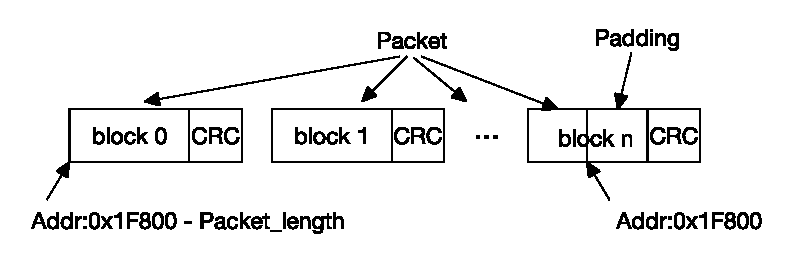
\includegraphics[width=0.6\textwidth]{./26-SDIOSLAVE/figures/SDIO_BUS_Packet_tran.eps}}
    \caption{SDIO 总线上数据传输}
    \label{figure:SDIO_BUS_Packet_tran}
\end{figure}

传输使用的是 IO\_RW\_EXTENDED (CMD53) 命令，其组成如图 \ref{figure:CMD53内容}，各部分具体含义请查看 SDIO 协议。

 \begin{figure}[H]
    \centering
    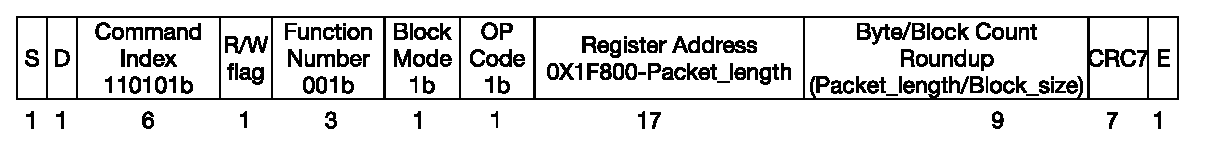
\includegraphics[width=0.9\textwidth]{./26-SDIOSLAVE/figures/CMD53_Content.eps}
    \caption{CMD53 内容}
    \label{figure:CMD53内容}
\end{figure}

\subsection{寄存器访问}

为了方便 Host 与 Slave 之间的信息交互，Host 可以通过 SDIO bus I/O Function1 访问 Slave 中的特定寄存器。这些寄存器在 \hyperref[regdesc:SLC0HOSTTOKENRDATA]{SLC0HOST\_TOKEN\_RDATA} 到 S\hyperref[regdesc:SLC0HOSTINTSTREG]{SLC0HOST\_INT\_ST\_REG} 的连续地址段内。Host 访问时只需将 CMD52 或 CMD53 中的寄存器地址设置为对应寄存器地址的低 10 位。Host 可以使用 CMD53 同时访问多个寄存器，提高了数据传输的速率。

SLCHOST\_CONF\_W0\_REG 到 SLCHOST\_CONF\_W15\_REG 共有 52 个字节的区域，Host 和 Slave 可以任意访问和修改，方便了 Host 与 Slave 之间的信息交互。

\subsection{DMA}

SDIO Slave 有一个专门的 DMA 用于从 RAM 获取或存储传输数据。如图 \ref{figure:SDIO Slave block diagram} 所示，DMA 通过 AHB 访问 RAM。DMA 使用链表结构来访问 RAM。每个链表由 3 个字 (word) 组成，具体结构如图 \ref{figure:链表结构} 所示。

 \begin{figure}[H]
    \centering
    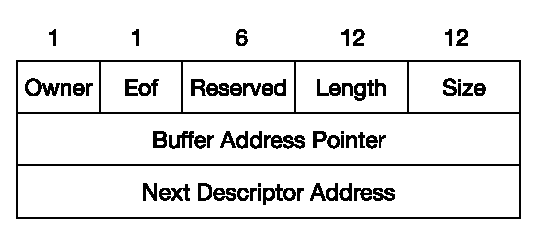
\includegraphics[width=0.4\textwidth]{./26-SDIOSLAVE/figures/Descriptor.eps}
    \caption{SDIO Slave DMA 链表结构}
    \label{figure:链表结构}
\end{figure}

 \begin{itemize}
    \item Owner：当前链表对应 buffer 允许的操作者。

             0：允许的操作者为 CPU

             1：允许的操作者为 DMA
    \item Eof：结束标志，表明当前链表是数据包的最后一个链表。
    \item Length：Buffer 中的有效字节数，即从 buffer 中能够被读取的字节数。
    \item Size：Buffer 允许使用的最大字节数。
    \item Buffer Address Pointer：Buffer 地址指针。
    \item Next Descriptor Address： 下一个链表的地址指针。当当前链表已经是最后一个链表时，Eof 位的值应为 1，该值应为 0。
\end{itemize}

Slave 链表串如图 \ref{figure:链表串} 所示：

 \begin{figure}[H]
    \centering
    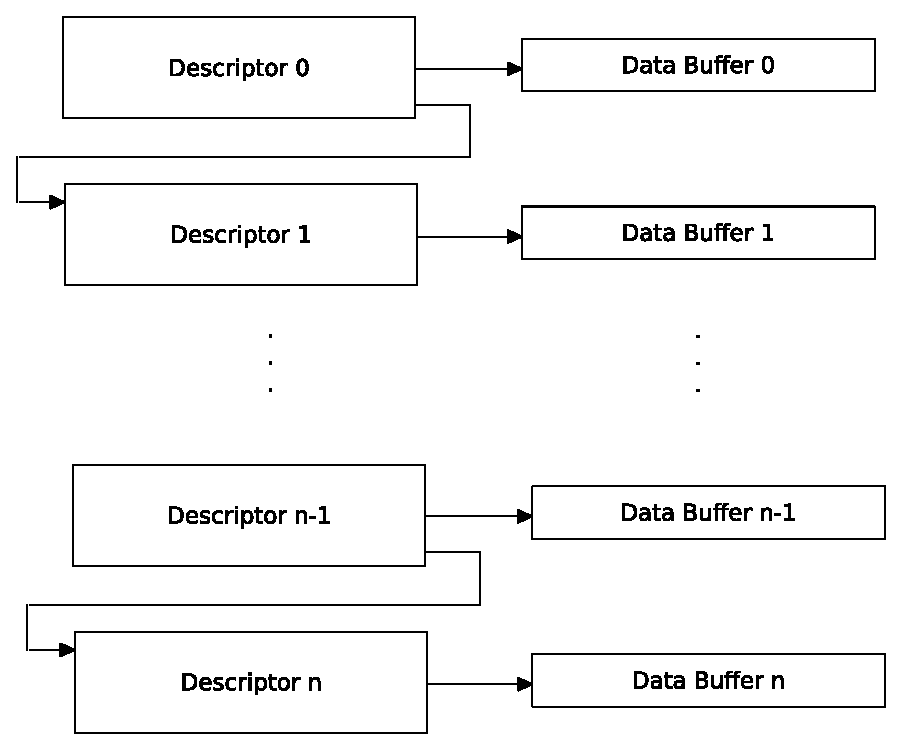
\includegraphics[width=0.6\textwidth]{./26-SDIOSLAVE/figures/Descriptor_chain}
    \caption{链表串}
    \label{figure:链表串}
\end{figure}

\subsection{包的发送和接收流程}
Host 与 Slave 间的包传输需要两者按照特定的流程配合完成。
\subsubsection{Slave 向 Host 发送包}
包的发送是由 Slave 发起，通过中断来通知 Host（中断实现方式参看 SDIO 协议）。Host 从 Slave 读取相关信息后发起 SDIO 总线传输。整个流程如图 \ref{figure:包的发送流程} 所示：


 \begin{figure}[H]
    \centering
    \fbox{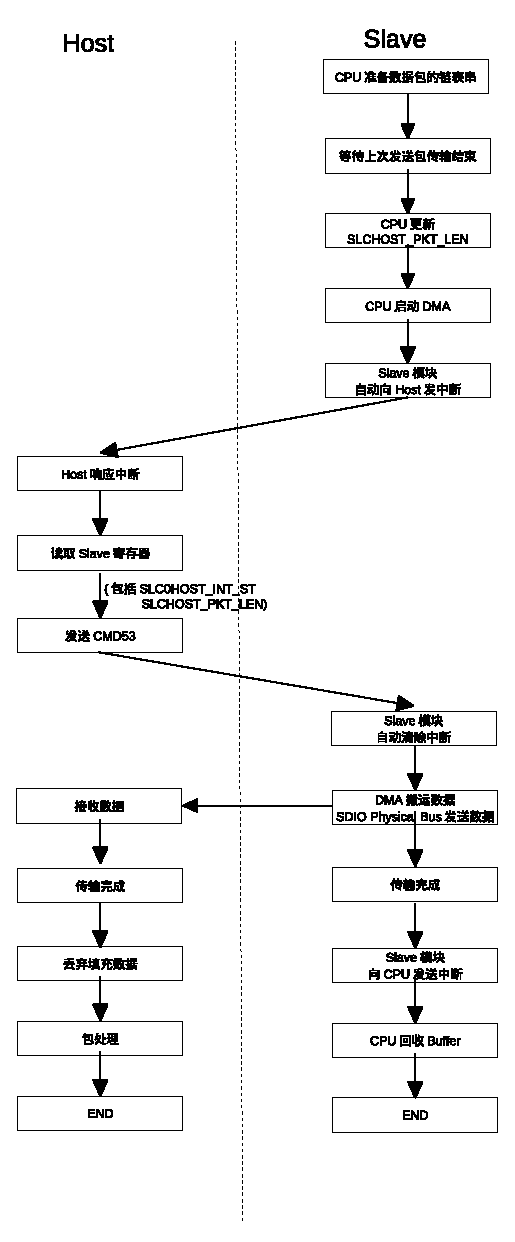
\includegraphics[width=0.55\textwidth]{./26-SDIOSLAVE/figures/Transition_flow.eps}}
    \caption{Slave 向 Host 发送包的流程}
    \label{figure:包的发送流程}
\end{figure}

 Host 从 Slave 读取相关信息是通过访问 SLC0HOST\_INT 和 SLCHOST\_PKT\_LEN 这两个寄存器实现的。


\begin{itemize}
    \item SLC0HOST\_INT：中断状态寄存器，其中 bit SLC0\_RX\_NEW\_PACKET\_INT\_ST 为 1 表明中断的原因是 Slave 发包。
    \item SLCHOST\_PKT\_LEN：Slave 发送包长度累加寄存器，Host 用本次读取值减去上次读取值就可以得到本次发送包的长度。
\end{itemize}

CPU 启动 DMA 需要先将链表串第一个链表的地址低 20 位写到寄存器 SLC0RX\_LINK 的 SLC0\_RXLINK\_ADDR 中，再配置 SLC0RX\_LINK 的 SLC0\_RXLINK\_START 来启动 DMA。之后 DMA 会自动完成数据的传输。

发送完成后 DMA 会向 CPU 发送中断，这时 CPU 可以回收 buffer。

\subsubsection{Slave 从 Host 接收包}
包的接收是由 Host 发起，Slave 通过 DMA 接收数据并存储到 RAM 中，传输完成后通过中断通知 CPU 进行数据处理。整个流程如图 \ref{figure:包的接收流程} 所示：

 \begin{figure}[H]
    \centering
    \fbox{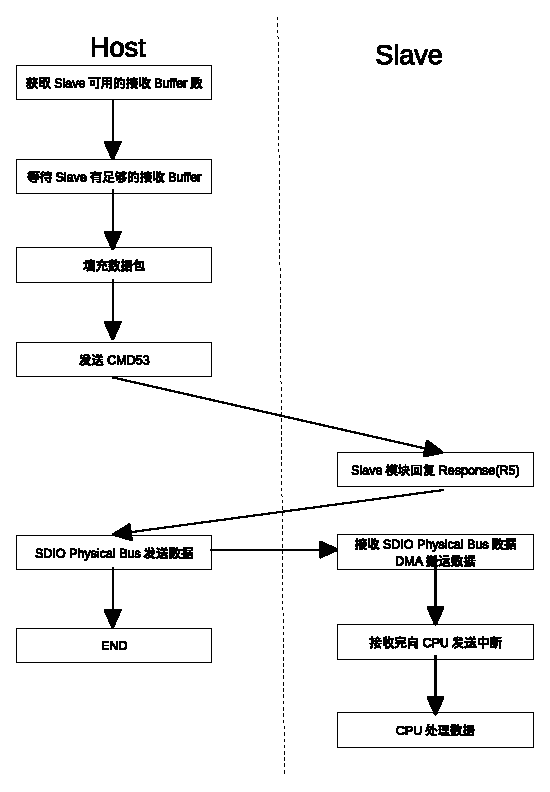
\includegraphics[width=0.6\textwidth]{./26-SDIOSLAVE/figures/Receive_flow.eps}}
    \caption{Slave 从 Host 接收包的流程}
    \label{figure:包的接收流程}
\end{figure}


Host 通过访问寄存器 SLC0HOST\_TOKEN\_RDATA 获取 Slave 侧可用于接收包的 buffer 数。Slave 侧的 CPU 要在准备好用于接收包的 DMA 链表后更新这个值。

SLC0HOST\_TOKEN\_RDATA 中 HOSTREG\_SLC0\_TOKEN1  存放可用 buffer 的累计值。

Host 通过 HOSTREG\_SLC0\_TOKEN1 减去自己已用掉的 buffer 数就得到了当前可用的 buffer 数。

当 buffer 不够用时，Host 需要通过不停地访问这个寄存器直到 buffer 够用为止。

为了保证有充足的 buffer 来接收包，Slave 的 CPU 必须不停地在接收链表上挂载 buffer。挂载的流程如图 \ref{figure:接收Buffer的挂载} 所示。

  \begin{figure}[H]
    \centering
    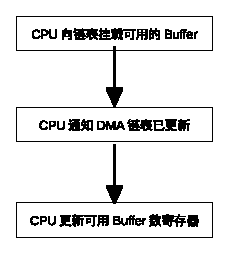
\includegraphics[width=0.27\textwidth]{./26-SDIOSLAVE/figures/Load_Buffer.eps}
    \caption{Slave CPU 挂载 buffer 的流程}
    \label{figure:接收Buffer的挂载}
\end{figure}

CPU 首先需要将新的 buffer 组成链表串并且挂载在 DMA 正在使用的链表串结尾。

然后 CPU 需要通知 DMA 链表串已更新，可以通过置位 SLC0TX\_LINK 寄存器的 SLC0\_TXLINK\_RESTART 为 1 来实现。注意，CPU 在首次启动 DMA 用于收包时需置位置 SLC0TX\_LINK 寄存器的 SLC0\_TXLINK\_START。

最后，CPU 通过配置 SLC0TOKEN1 寄存器更新可用的 buffer。

\subsection{SDIO 总线时序}\label{SDIO slave timing}
Host 与 Slave 间是通过 PCB 走线连接，所以延迟大。为了保证总线上时序正确，Slave 支持调整 SDIO 总线输入的采样时钟沿和输出的驱动时钟沿。

当从 Host 来的数据变化的时刻靠近时钟的上升沿时，Slave 会选择时钟的下降沿进行采样。采样时序图如图 \ref{figure:采样时序图} 所示：

 \begin{figure}[H]
    \centering
    \fbox{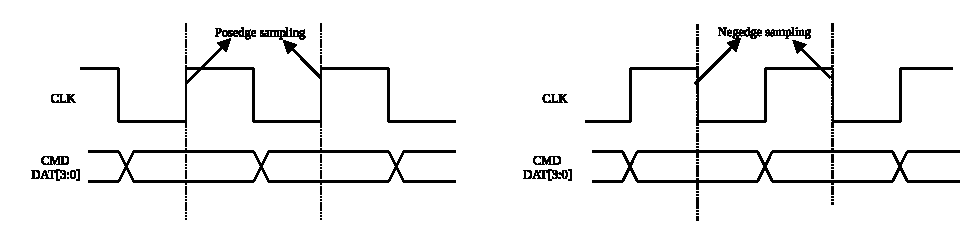
\includegraphics[width=0.9\textwidth]{./26-SDIOSLAVE/figures/Sampling.eps}}
    \caption{采样时序图}
    \label{figure:采样时序图}
\end{figure}

Slave 管脚采样沿默认由 MTDO strapping 值决定，但通过配置 \hyperref[regdesc:SLCHOSTCONFREG]{SLCHOST\_CONF\_REG} 寄存器可以强制决定模式（优先级从高到低）：(1) 置位 SLCHOST\_FRC\_POS\_SAMP，对应管脚强制上升沿采样；(2) 置位 SLCHOST\_FRC\_NEG\_SAMP，对应管脚强制下降沿采样。

SLCHOST\_FRC\_POS\_SAMP 和 SLCHOST\_FRC\_NEG\_SAMP 的位宽均为 5 bit，5 个 bit 分别对应 CMD 线和 4 个 DATA 线 (0-3)。置位这两个域使得 Slave 对相应的线在时钟上升沿或下降沿上进行采样。

Slave 还可以选择时钟的上升沿还是下降沿对数据输出线进行驱动，以适应不同的延迟。时序图如图 \ref{figure:输出时序图} 所示：
  \begin{figure}[H]
    \centering
    \fbox{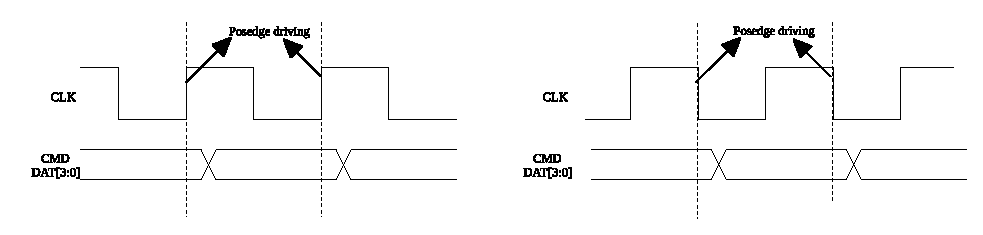
\includegraphics[width=0.9\textwidth]{./26-SDIOSLAVE/figures/Driving.eps}}
    \caption{输出时序图}
    \label{figure:输出时序图}
\end{figure}

Slave 管脚输出沿默认由 GPIO5 strapping 值决定 ，但通过配置以下寄存器可以强制决定模式（优先级从高到低）：(1) 置位 \hyperref[regdesc:SLCHOSTCONFREG]{SLCHOST\_CONF\_REG} 中的 SLCHOST\_FRC\_SDIO11，对应管脚强制下降沿输出； (2) 置位 \hyperref[regdesc:SLCHOSTCONFREG]{SLCHOST\_CONF\_REG} 中的 SLCHOST\_FRC\_SDIO22，对应管脚强制上升沿输出；(3) 置位 \hyperref[regdesc:HINFCFGDATA1REG]{HINF\_CFG\_DATA1\_REG} 中的 HINF\_HIGHSPEED\_ENABLE 和 \hyperref[regdesc:SLCHOSTCONFREG]{SLCHOST\_CONF\_REG} 中的 SLCHOST\_HSPEED\_CON\_EN 后，主机通过配置 CCCR 中的 EHS (Enable High-Speed) 为 1 强制上升沿输出。

SLCHOST\_FRC\_SDIO11 和 SLCHOST\_FRC\_SDIO22 的位宽均为 5 bit，5 个 bit 分别对应 CMD 线和 4 个 DATA 线 (0-3)。置位这两个域使得 Slave 在时钟下降沿或上升沿上对相应的线进行驱动。

{\bfseries 关于优先级的说明}：无论输入还是输出，strapping 管脚的配置也被包含在优先级范围内（优先级最低）。每一级有效的前提是比它高的优先级都不生效。例如 MTDO strapping 的配置决定对应管脚的采样沿，生效的前提是 SCLHOST\_FRC\_POS\_SAMP 没有置 1，SCLHOST\_FRC\_NEG\_SAMP 也没有置 1。

\subsection{中断}
Host 和 Slave 间可以通过配置中断向量灵活地中断对方。Host 和 Slave 各有 8 个中断向量可用于中断对方。在配置中断向量寄存器后就会向对方发送中断（配置相应的中断使能寄存器）。中断向量寄存器具有自清功能，所以配置一次会产生一次中断，不需要其他操作。

\subsubsection{Host 侧中断}
\begin{itemize}
\item {\it SLC0HOST\_SLC0\_RX\_NEW\_PACKET\_INT\label{int:SLC0HOSTSLC0RXNEWPACKETINT}} Slave 发包中断
\item {\it SLC0HOST\_SLC0\_TX\_OVF\_INT\label{int:SLC0HOSTSLC0TXOVFINT}} Slave 接收 buffer 溢出中断
\item {\it SLC0HOST\_SLC0\_RX\_UDF\_INT\label{int:SLC0HOSTSLC0RXUDFINT}} Slave 发送 buffer 下溢中断
\item {\it SLC0HOST\_SLC0\_TOHOST\_BIT\textcolor{red}{\it{n}}\_INT\label{int:SLC0HOSTSLC0TOHOSTBITnINT}} (\textcolor{red}{\it{n}}: 0 \verb+~+ 7) Slave 中断 Host
\end{itemize}

\subsubsection{Slave 侧中断}
\begin{itemize}
\item {\it SLC0INT\_SLC0\_RX\_DSCR\_ERR\_INT} Slave 发送描述符错误中断
\item {\it SLC0INT\_SLC0\_TX\_DSCR\_ERR\_INT} Slave 接收描述符错误中断
\item {\it SLC0INT\_SLC0\_RX\_EOF\_INT} Slave 发送操作完成中断
\item {\it SLC0INT\_SLC0\_RX\_DONE\_INT} 单个 buffer 由 Slave 发送完成的中断
\item {\it SLC0INT\_SLC0\_TX\_SUC\_EOF\_INT} Slave 接收操作完成中断
\item {\it SLC0INT\_SLC0\_TX\_DONE\_INT} A 单个 buffer 在 Slave 接收操作时填满了的中断
\item {\it SLC0INT\_SLC0\_TX\_OVF\_INT} Slave 接收 buffer 溢出中断
\item {\it SLC0INT\_SLC0\_RX\_UDF\_INT} Slave 发送 buffer 下溢中断
\item {\it SLC0INT\_SLC0\_TX\_START\_INT} Slave 接收操作开始中断
\item {\it SLC0INT\_SLC0\_RX\_START\_INT} Slave 发送操作开始中断
\item {\it SLC0INT\_SLC\_FRHOST\_BIT\textcolor{red}{\it{n}}\_INT\label{int:SLC0INTSLCFRHOSTBITnINT}} (\textcolor{red}{\it{n}}: 0 \verb+~+ 7) Host 中断 Slave
\end{itemize}

\hypertarget{sdioslave-reg-summ}{}
\section{寄存器列表}\label{sec:sdioslave-reg-summ}

本小节的所有地址均为相对于 SDIO 从机基地址的地址偏移量（相对地址），具体基地址请见章节 \ref{mod:sysmem} \textit{\nameref{mod:sysmem}} 中的表 \ref{table:Peripheral_Address_Mapping}。

请查看章节 \hyperref[glossary-access-types]{\textit{寄存器的访问类型}}，了解“访问”列缩写的含义。

\subfile{\modulefiles/sdioslave_reg-summary_cn}

{\clearpage}
\section{SLC 寄存器}

本小节的所有地址均为相对于 SDIO 从机基地址 (0x3FF5\_8000) 的地址偏移量（相对地址），具体基地址请见章节 \ref{mod:sysmem} \textit{\nameref{mod:sysmem}} 中的表 \ref{table:Peripheral_Address_Mapping}。寄存器绝对地址见章节 \ref{sec:sdioslave-reg-summ} \textit{\nameref{sec:sdioslave-reg-summ}}。

关于保留 (reserved) 域的处理，请查看章节 \hyperref[programming-reserved-field]{\textit{如何配置寄存器的保留域}}。

\subfile{\modulefiles/slc_reg_cn.tex}

\section{SLC Host 寄存器}

本小节的所有地址均为相对于 SDIO 从机基地址 (0x3FF5\_5000) 的地址偏移量（相对地址），具体基地址请见章节 \ref{mod:sysmem} \textit{\nameref{mod:sysmem}} 中的表 \ref{table:Peripheral_Address_Mapping}。寄存器绝对地址见章节 \ref{sec:sdioslave-reg-summ} \textit{\nameref{sec:sdioslave-reg-summ}}。

关于保留 (reserved) 域的处理，请查看章节 \hyperref[programming-reserved-field]{\textit{如何配置寄存器的保留域}}。


\subfile{\modulefiles/host_reg_cn.tex}

\section{HINF 寄存器}

本小节的所有地址均为相对于 SDIO 从机基地址 (0x3FF4\_B000) 的地址偏移量（相对地址），具体基地址请见章节 \ref{mod:sysmem} \textit{\nameref{mod:sysmem}} 中的表 \ref{table:Peripheral_Address_Mapping}。寄存器绝对地址见章节 \ref{sec:sdioslave-reg-summ} \textit{\nameref{sec:sdioslave-reg-summ}}。

关于保留 (reserved) 域的处理，请查看章节 \hyperref[programming-reserved-field]{\textit{如何配置寄存器的保留域}}。

\subfile{\modulefiles/hinf_reg_cn.tex}

\end{document}
